\chapter{Analysis}

\section{Introduction}

\subsection{Client Identification} 
My client is Tom Wolf, he is 46 years old and he is my A level ICT teacher. Tom teaches A level ICT, Doploma ICT and GCSE ICT at Long Road sixth form college. As he is an ICT teacher, he is very educated in computer related subjects, but his programming experience is relatively small and he is not able to write complex programs for himself.

\subsection{Define the current system} 
Currently the system is Tom himself and Google Drive and his hard drive on his laptop used to store calculated data. Tom is required to collect grades of students from the school system, use an algorithm to calculate his students predicted grades, create a table using already purcheased software such as Microsoft Word and  insert new calculated data to the table. This is very time consuming, as he is required to repeat this process after few assignments for all his students, which is every 2-3 weeks.

\subsection{Section appendix}

Summerised Interview

What sort of system do you need currently?
-It has to be an electronic equivalent of a markbook
-It should be able to store infinite amount of units, which represent a term (spring term, autumn term,etc)
-Within the units should be assignments
-Assignments represent exams, school work, tests grades, etc.
-The number of assignments within a unit also shouldn't have limitation
-Predicted grade should be calculated in the program, for an assignment a maximum mark should be assigned and for every student, a mark should be given
-Using a specific algotithm, a grade should be calculated
-Using the grades from the assignments, a predicted grade for the end of the unit and the end of the year should be calculated
-The system should also be capable of calculating the average grade for the whole class for the assignment, unit, and the average predicted grade for the whole class.
-Additionally, it is not required, the system should have a function to calculate the average predicted grade for the whole year
-Calculating the grade for A2 and AS should use a different algorithm

\subsection{Describe the problems}

Tom is required to calculate predicted grades for 200 students by himself and this requires his own time, so the school does not pay him for this. So, for Tom this is not satisfactory as 200 students is a big amount and so it requires a lot of effort and time. Therefore, Tom requires software that will perform those calculations automatically. 

\section{Investigation}

\subsection{The current system}
\subsubsection{Data sources and destinations}

\begin{figure}[H]
    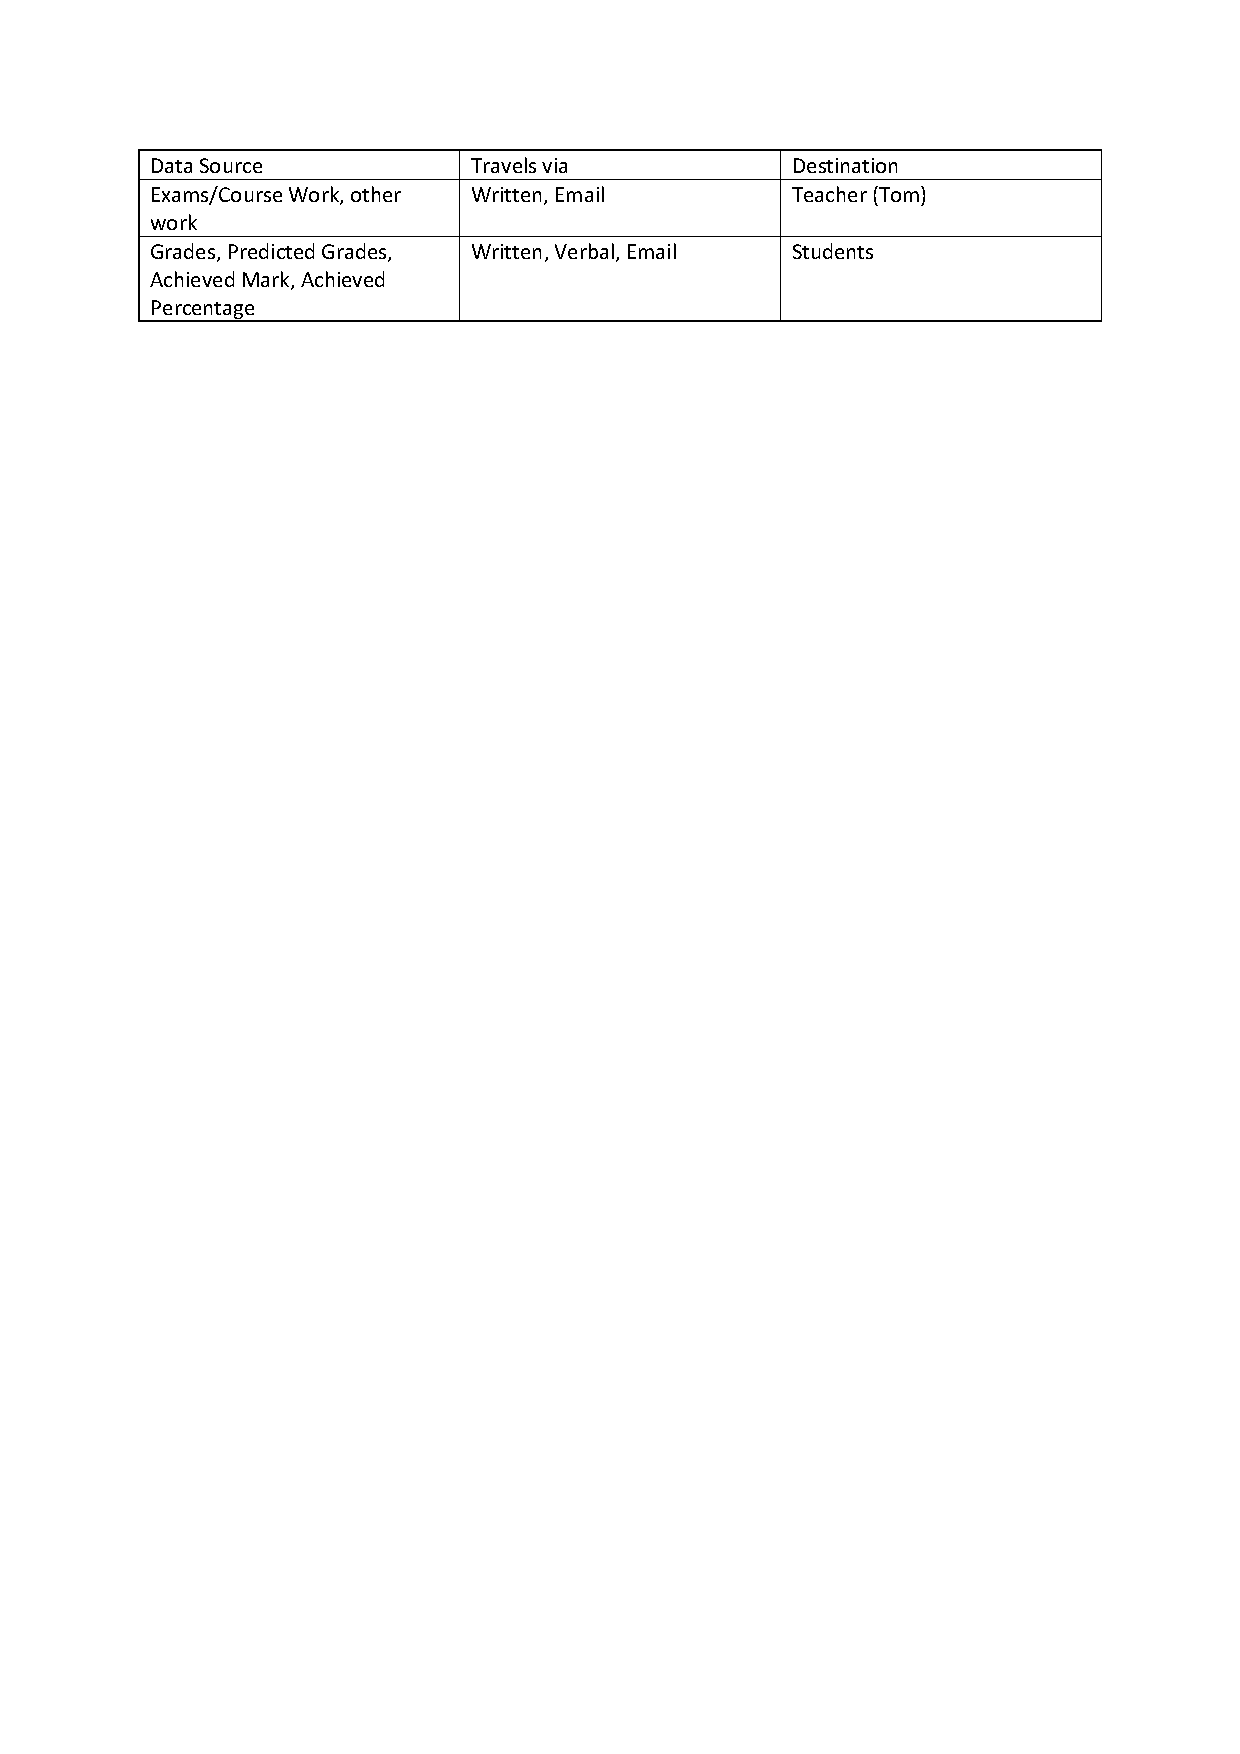
\includegraphics[width=\textwidth]{./Analysis/images/DataSourcesandDestinations.pdf}
\end{figure}


\subsubsection{Algorithms}
At this point I am aware of the following algorithms:
-Calculating the end of the unit predicted grade


-Calculating the end of the unit predicted grade

\begin{algorithm}[H]
\SET{$Score$}{$0$}
\For{$grade$}{$Assignment$}
     \If{$grade = "A*"$}
          \Set{$Score$}{$Score+6$}
     \ElsIf{$grade = "A"$}
          \Set{$Score$}{$Score+5$}
     \ElsIf{$grade = "B"$}
          \Set{$Score$}{$Score+4$}
     \ElsIf{$grade = "C"$}
          \Set{$Score$}{$Score+3$}
     \ElsIf{$grade = "D"$}
          \Set{$Score$}{$Score+2$}
     \ElsIf{$grade = "E"$}
          \Set{$Score$}{$Score+1$}
\EndFor
\SET{$Score$}{$Score / length(assignments)$}

\If{$Score > 5.5$}
     \Set{$Score$}${EndOfUnitG = "A*"$}
\ElsIf{$Score > 4.5$}
     \Set{$Score$}{$EndOfUnitG = "A"$}
\ElsIf{$Score > 3.5$}
     \Set{$Score$}{$EndOfUnitG = "B"$}
\ElsIf{$Score > 2.5$}
     \Set{$Score$}{$EndOfUnitG = "C"$}
\ElsIf{$Score > 1.5$}
     \Set{$Score$}{$EndOfUnitG = "D"$}
\ElsIf{$Score > 0.5$}
     \Set{$Score$}{$EndOfUnitG = "E"$}
\Else
     \Set{$Score$}{$EndOfUnitG = "U"$}
\end{algorithmic}
\end{algorithm}
-Calculating the end of the year predicted grade(for AS)

\begin{algorithm}[H]
\SET{$Score$}{$0$}
\For{$grade$}{$Unit$}
     \If{$grade = "A*"$}
          \Set{$Score$}{$Score+6$}
     \ElsIf{$grade = "A"$}
          \Set{$Score$}{$Score+5$}
     \ElsIf{$grade = "B"$}
          \Set{$Score$}{$Score+4$}
     \ElsIf{$grade = "C"$}
          \Set{$Score$}{$Score+3$}
     \ElsIf{$grade = "D"$}
          \Set{$Score$}{$Score+2$}
     \ElsIf{$grade = "E"$}
          \Set{$Score$}{$Score+1$}
\EndFor
\SET{$Score$}{$Score / length(units)$}

\If{$Score > 5.5$}
     \Set{$Score$}${ASPredictedG = "A*"$}
\ElsIf{$Score > 4.5$}
     \Set{$Score$}{$ASPredictedG = "A"$}
\ElsIf{$Score > 3.5$}
     \Set{$Score$}{$ASPredictedG = "B"$}
\ElsIf{$Score > 2.5$}
     \Set{$Score$}{$ASPredictedG = "C"$}
\ElsIf{$Score > 1.5$}
     \Set{$Score$}{$ASPredictedG = "D"$}
\ElsIf{$Score > 0.5$}
     \Set{$Score$}{$ASPredictedG = "E"$}
\Else
     \Set{$Score$}{$ASPredictedG = "U"$}
\end{algorithmic}
\end{algorithm}

-Calculating the end of the year predicted grade (for AS)

-Calculating end of the year predicted grade(for A2)

-Calculating the grade

\begin{algorithm}[H]
\Set{$percent$}{$(AchievedMark / MaxMark) * 100$}
\If{$percent > "90"$}
       \SET{$grade$}{$A*$}
\ElsIf{$percent = "80"$}
       \Set{$grade$}{$A$}
\ElsIf{$percent = "70"$}
       \Set{$grade$}{$B$}
\ElsIf{$percent = "60"$}
       \Set{$grade$}{$C$}
\ElsIf{$percent = "50"$}
       \Set{$grade$}{$D$}
\ElsIf{$percent = "40"$}
       \Set{$grade$}{$E$}
\Else
       \Set{$grade$}{$U$}
\end{algorithmic}
\end{algorithm}

-Calculating average predicted end of the year grade for the whole class

-Calculating average predicted  end of the unit grade for the whole class

-Calculating average end of the year grade for the whole class



\subsubsection{Data flow diagram}

\begin{figure}[H]
    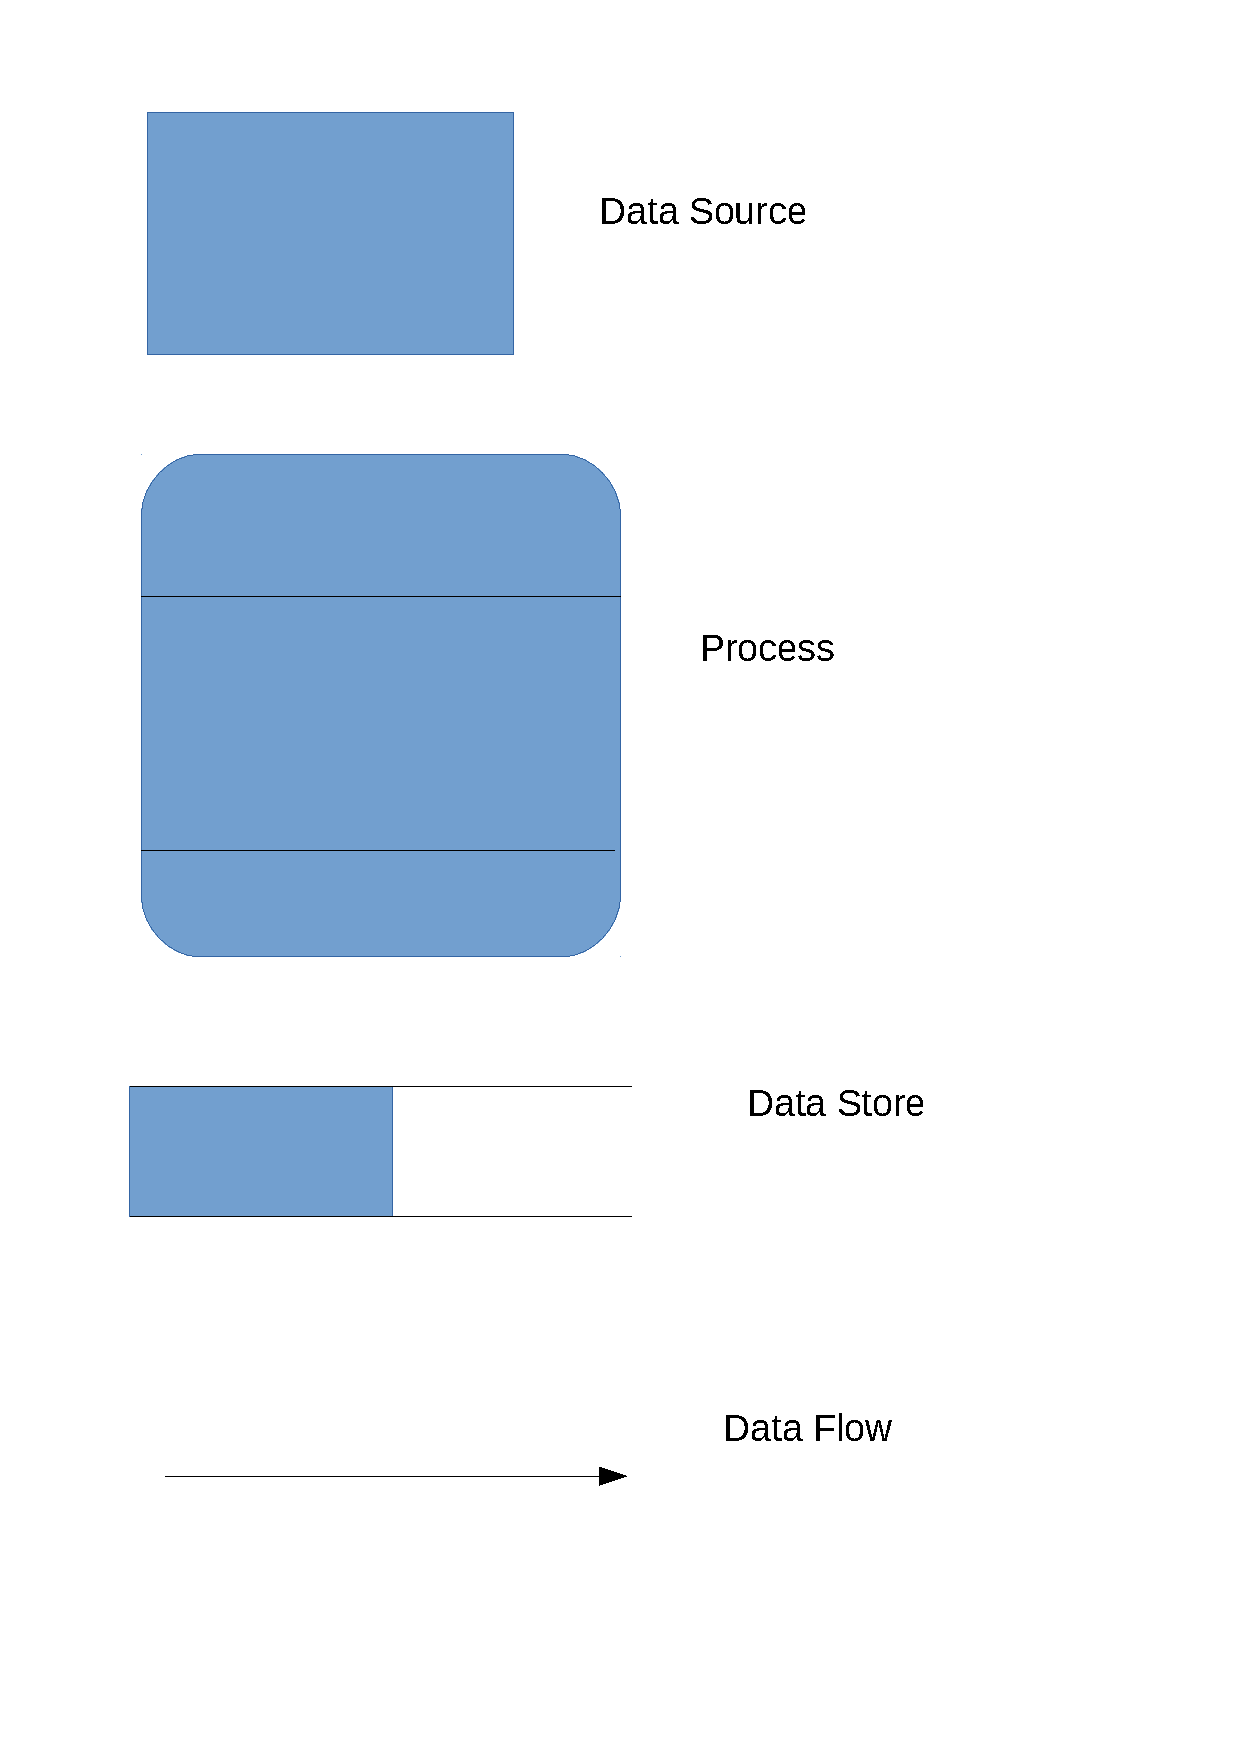
\includegraphics[width=\textwidth]{./Analysis/images/key.pdf}
    \caption{This is the key for the following data flow diagrams.} \label{fig:data_flow_diagram_key}
\end{figure}

\begin{figure}[H]
    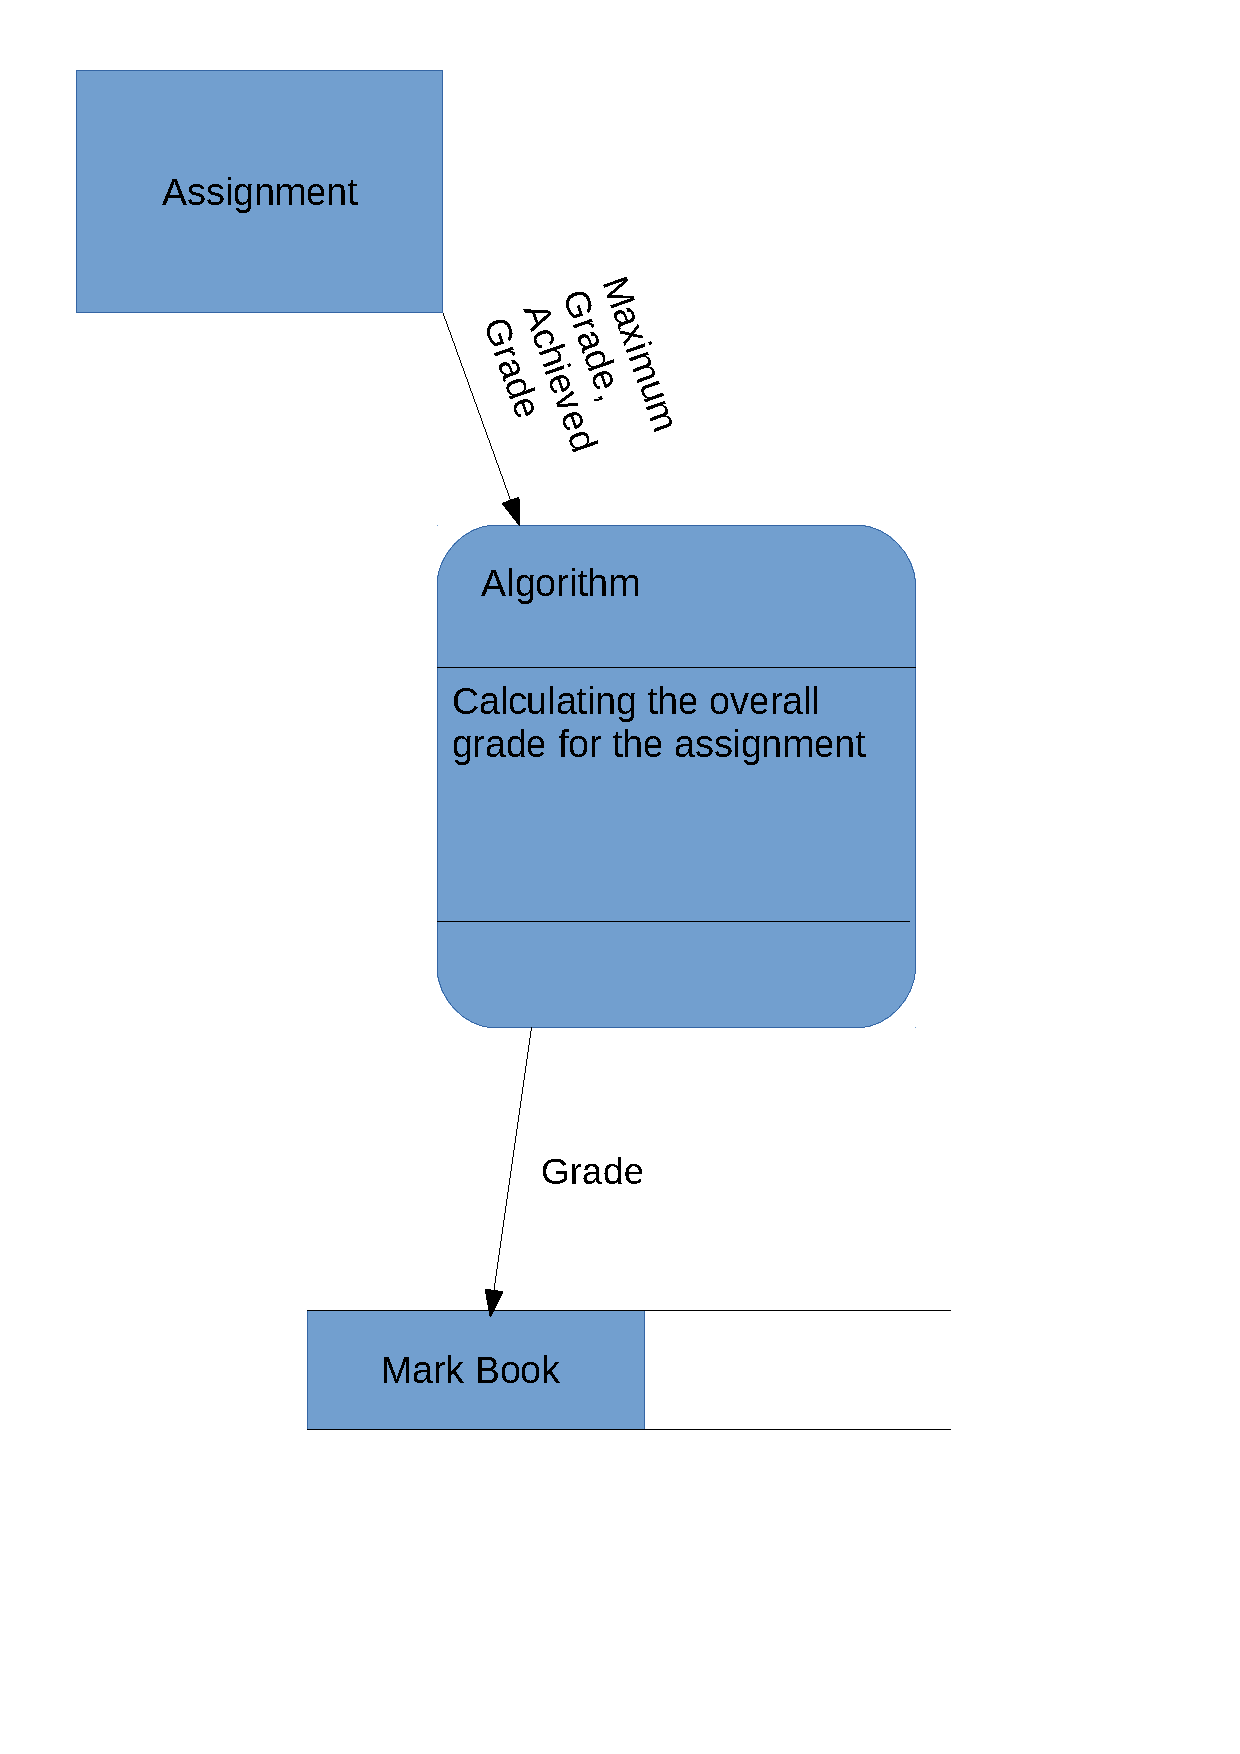
\includegraphics[width=\textwidth]{./Analysis/images/DataFlowDiagrams.pdf}
\end{figure}

\begin{figure}[H]
    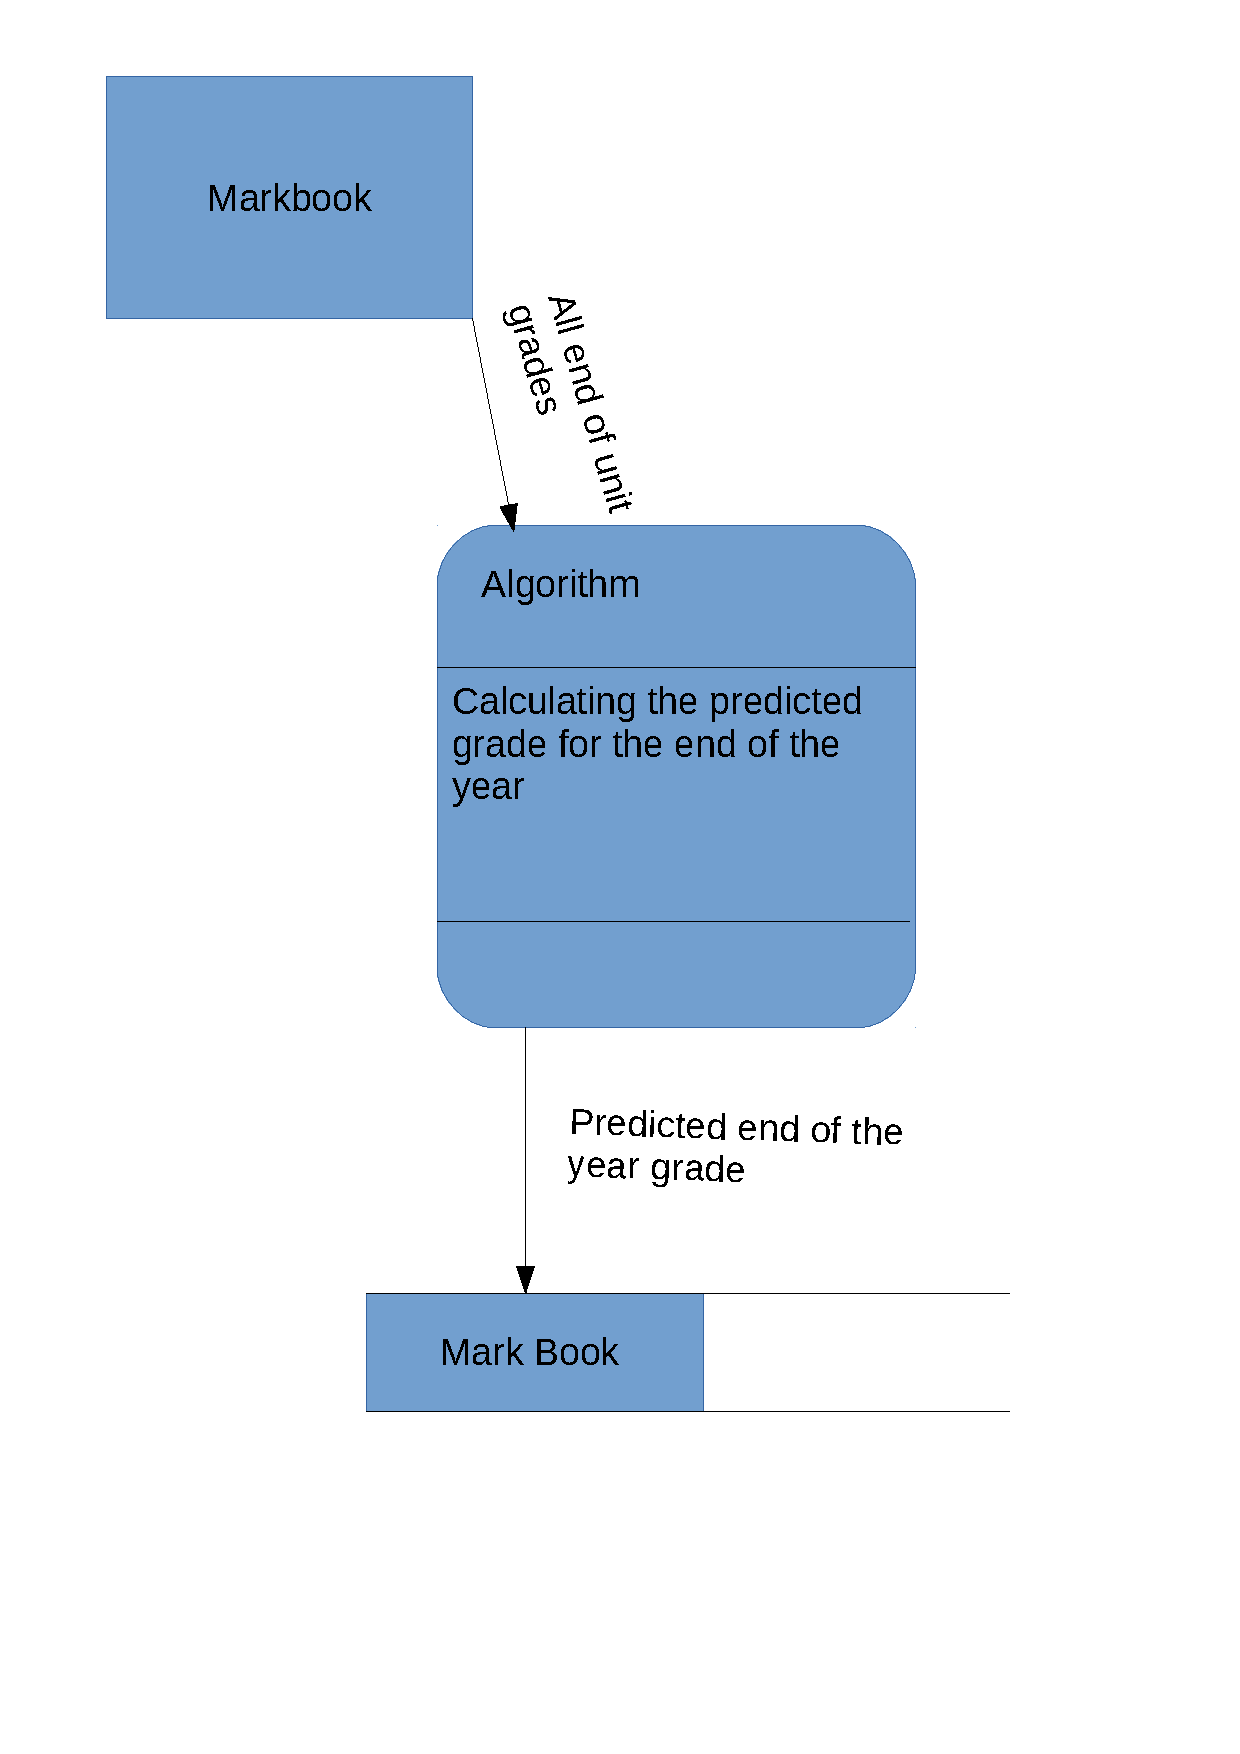
\includegraphics[width=\textwidth]{./Analysis/images/DataFlowDiagrams2.pdf}
\end{figure}

\subsubsection{Input Forms, Output Forms, Report Formats}

In the current system, students' work is an input form for Tom's students; based on this, Tom is able to calculate students' grades for assignments, from which he is then able to calculate other predicted grades, such as predicted end of the year grade and end of the unit grade.

(This section is not fully finished)

\subsection{The proposed system}

\subsubsection{Data sources and destinations}

In the proposed system, the data sources and destinations are exactly the same as in the current system, the only difference will be that the data which Tom had to calculate manually with now be done automatically by the proposed system.

\begin{figure}[H]
    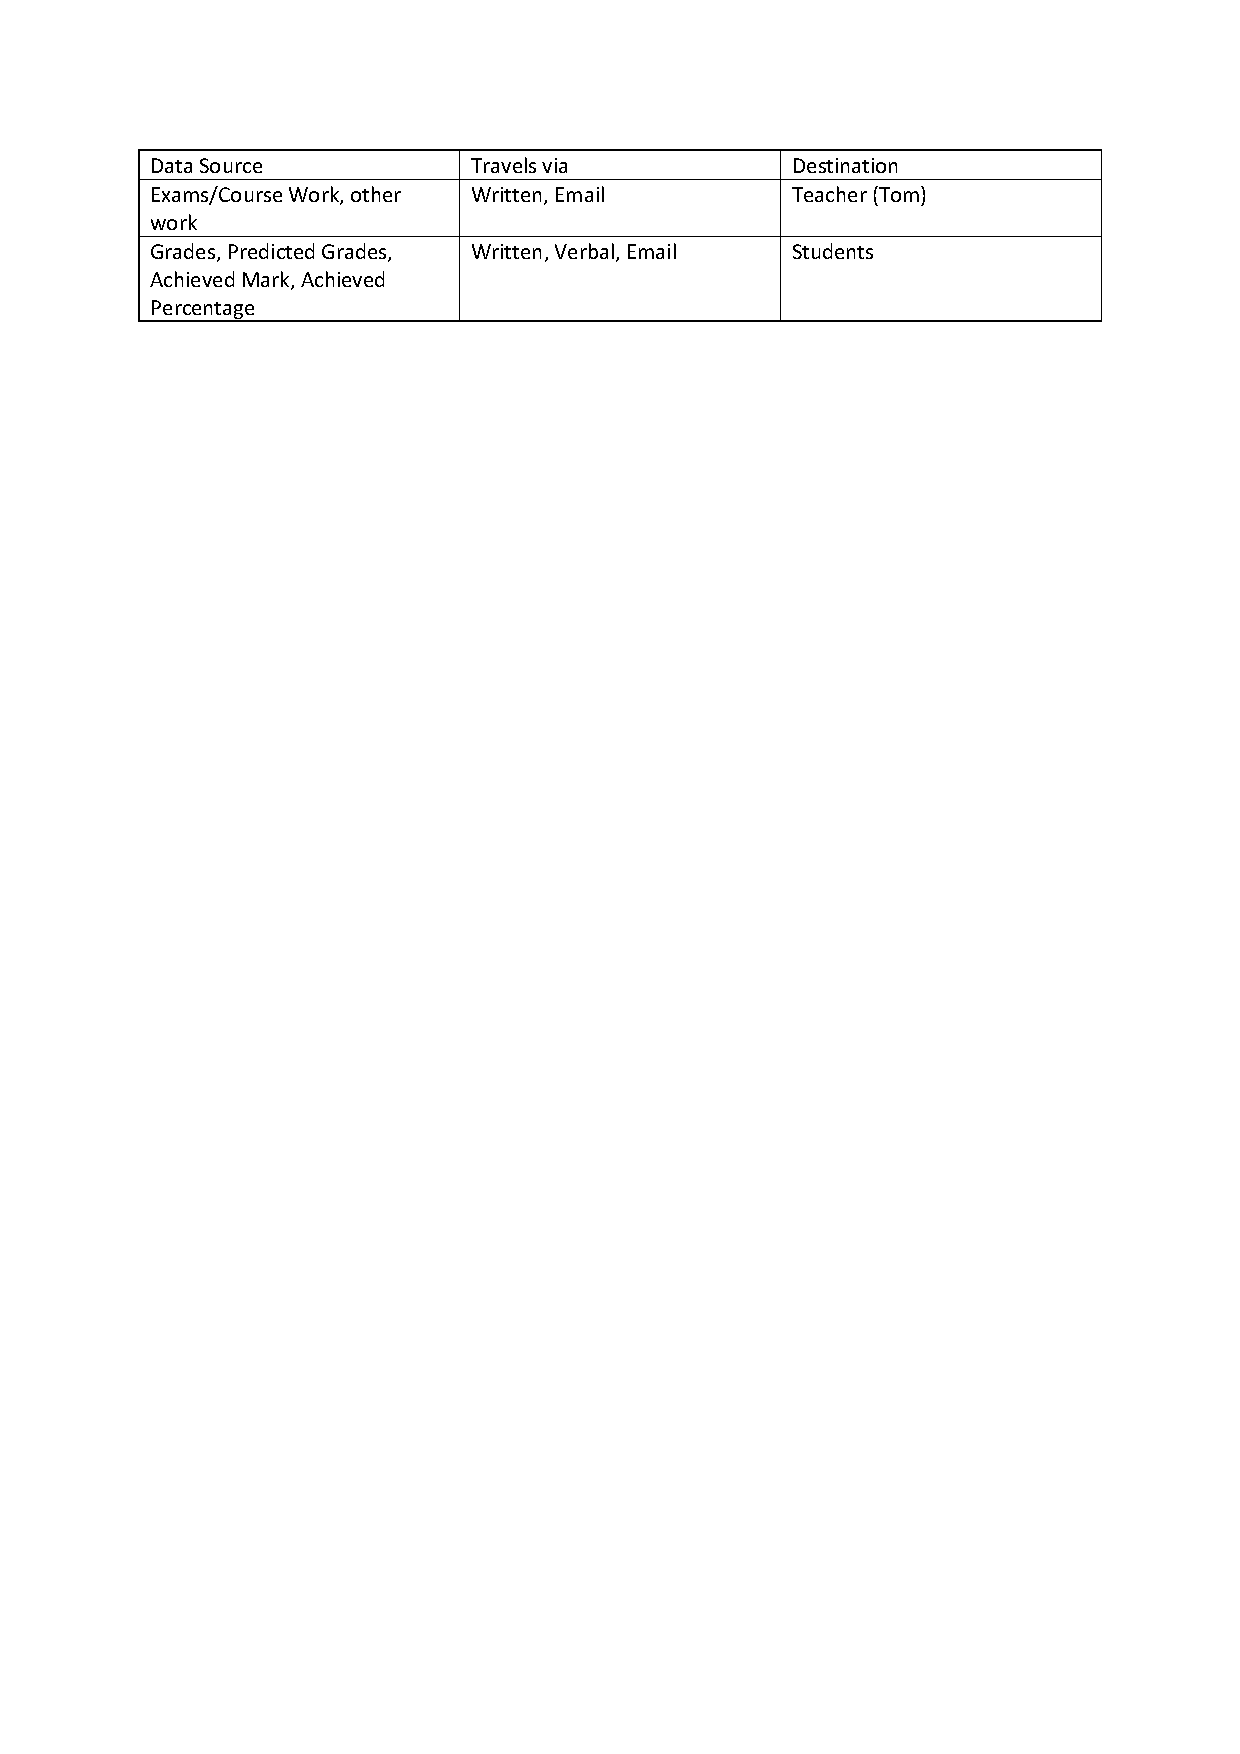
\includegraphics[width=\textwidth]{./Analysis/images/DataSourcesandDestinations.pdf}
\end{figure} 

\subsubsection{Data flow diagram}

\begin{figure}[H]
    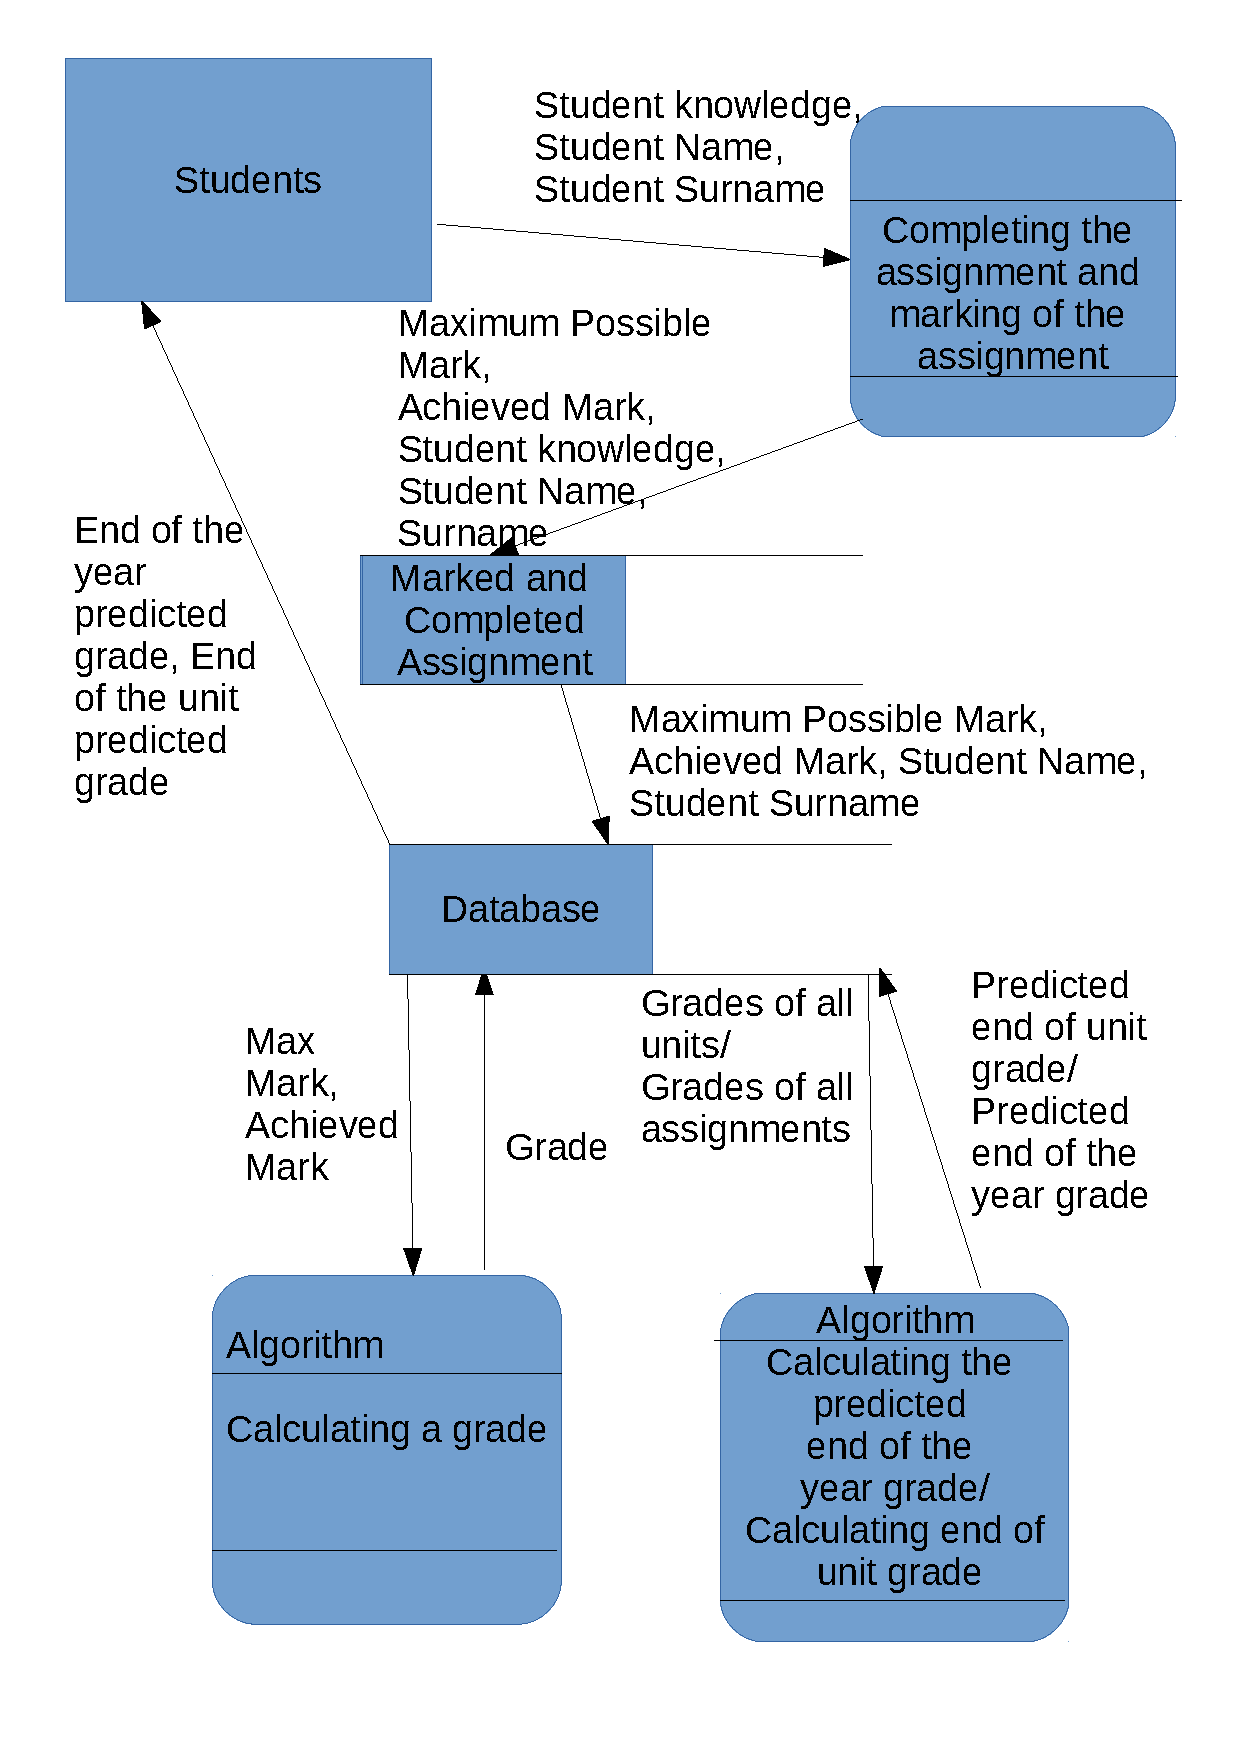
\includegraphics[width=\textwidth]{./Analysis/images/222DataFlowDiagram.pdf}
\end{figure}

\subsubsection{Data dictionary}
\begin{figure}[H]
    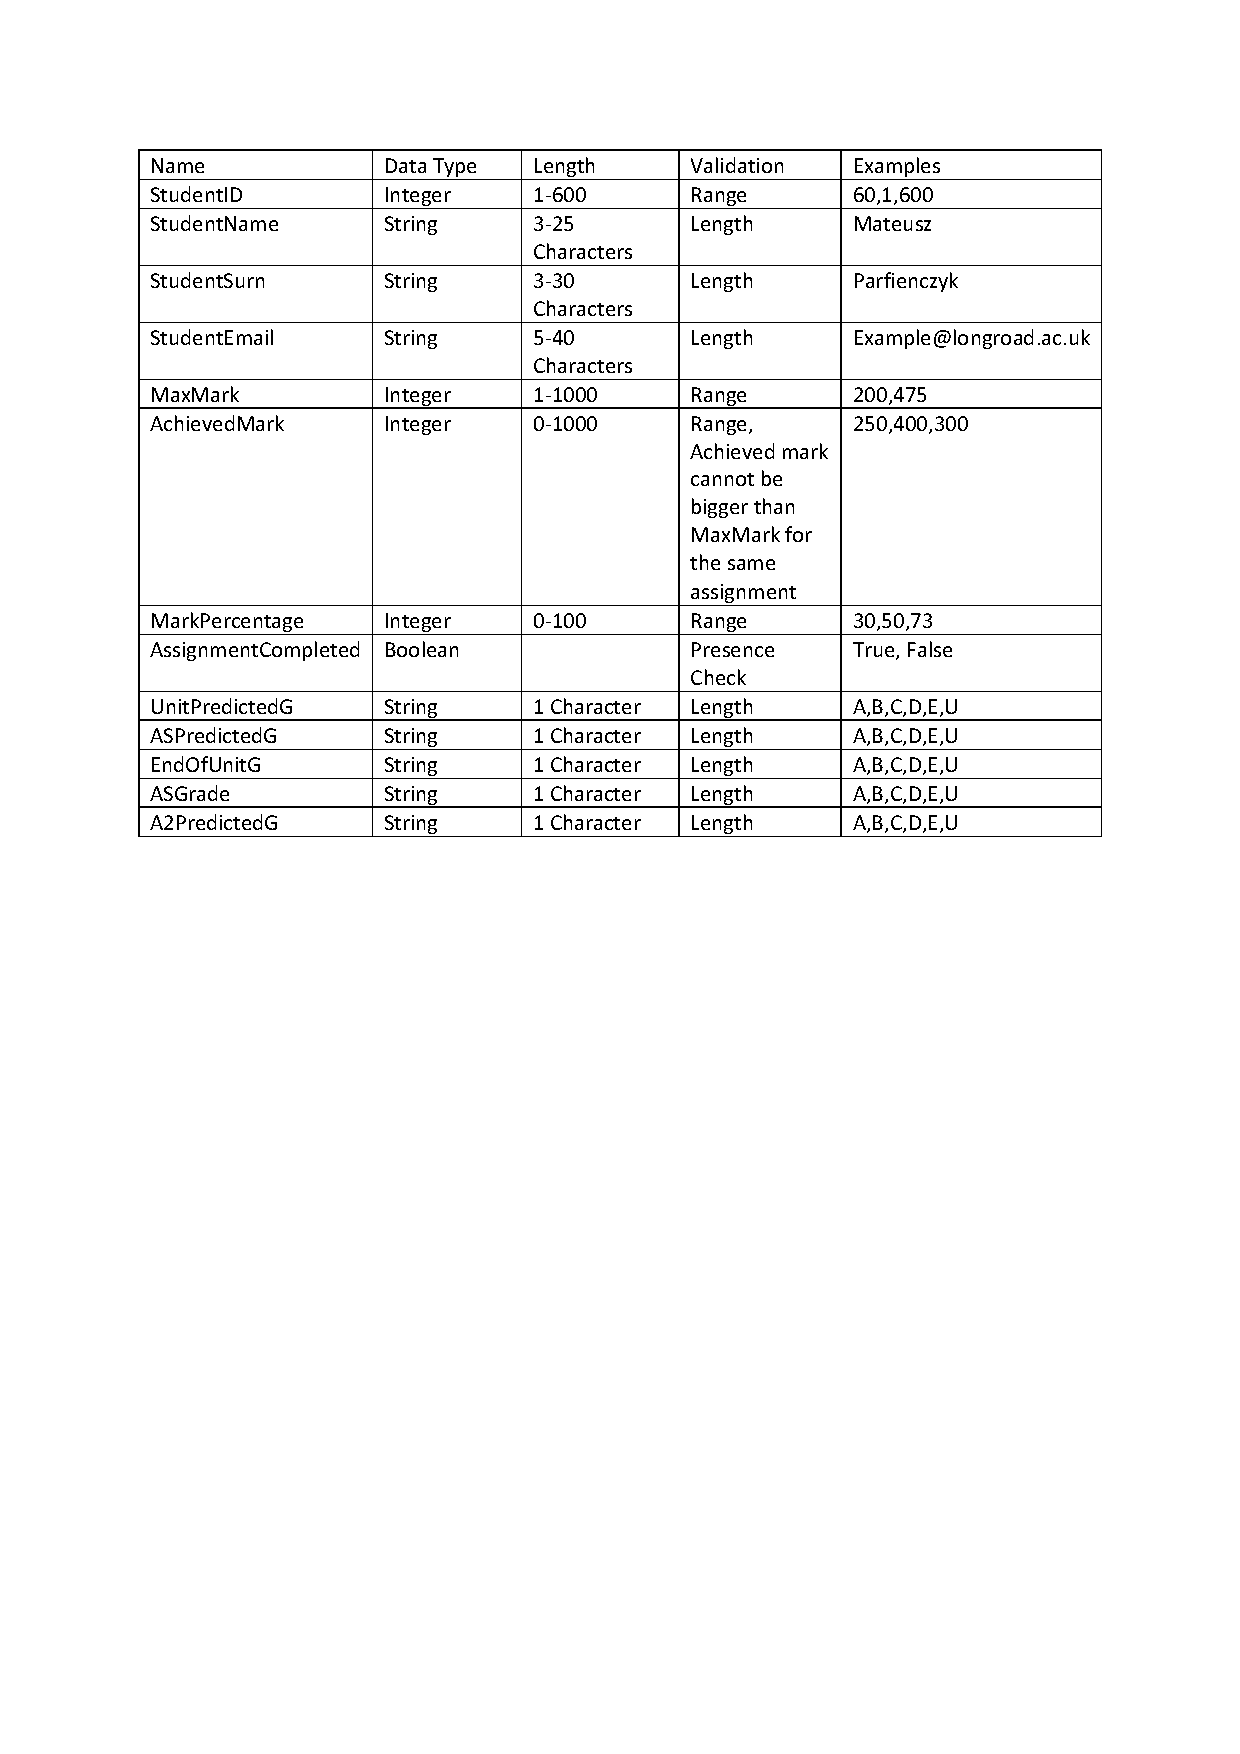
\includegraphics[width=\textwidth]{./Analysis/images/DataDictionary.pdf}
\end{figure}

\subsubsection{Volumetrics}
The system should be able to store at least 200 students' data because that is the number of students Tom teaches at Long Road. 
So to prevent issues related to data storage, I propose that the amount of reserved storage should at least be double of that.

\section{Objectives}
\subsection{General Objectives}

The system should allow to insert grades for an assignment in alphabetical order for studenst, with an option either from A-Z or from Z-A for an ICT class. It should also be capable of inserting grades and predicted grades for multiple assignments for a selected student individually.

\subsection{Specific Objectives}

\subsection{Core Objectives}

\subsection{Other Objectives}

\section{ER Diagrams and Descriptions}

\subsection{ER Diagram}

\subsection{Entity Descriptions}

\section{Object Analysis}

\subsection{Object Listing}

\subsection{Relationship diagrams}

\subsection{Class definitions}

\section{Other Abstractions and Graphs}

\section{Constraints}

\subsection{Hardware}
Laptop: Core 2 Duo, 2Gb of RAM, 300Gb HDD, 17" display with a resolution 1920x720, intel integrated graphics, Windows 7 operating system.

Although the laptop is 6 years old and it will not be able to run complex programs released in past 2 years, although it is definitely capable of running Python with the PyQt4 extension.

\subsection{Software}

It would be a good addition to the program if it could import data and export data from the school system, so that Tom would not have to do this manually, which would require additional time for Tom to spend. Tom didn't state whether he would prefer or not prefer to use other software to alter data in the database and/or display it, although I know that Tom uses Excel for this sort storage, so it would be better if the system was compatible with other formatting.


\subsection{Time}
The very final deadline for this task to be finished is Friday 17th April, this date is set by my computing teacher, Adam McNicol. If I will complete the system earlier, it is unlikely that Tom is going to use it this school year. 

\subsection{User Knowledge}

As I mentioned in Client Identification, Tom has a lot of computer/IT experience, so he should be capable of using any system/program I will provide for him

\subsection{Access restrictions}
Because Tom has privilages to change student grades and predicted grades, the system should allow Tom to change those and also the system should be protected with a password or other form of security to prevent un-authorised access, such as students which have an intention of altering their grades.

\section{Limitations}

\subsection{Areas which will not be included in computerisation}
All of the marking has to be done by Tom, entering the mark also has to be done by Tom.

\subsection{Areas considered for future computerisation}
The student names, surnames and emails could possibly be imported from the school database/network. Also, the grades and predicted grades could be sent automatically with a capable of doing this system.

\section{Solutions}

\subsection{Alternative solutions}

I could write the program in python with the pyQt extension and install the database on internet, as it would be the most secure and Tom would not need to have the database file on his storage device as long as he would have access to internet.

\subsection{Justification of chosen solution}To complete this project, I will use Python and PyQT python extension/module because I learned the basics of Python in AS computing and I am continuing computing this year, so my Python programming skills will also improve throughout the year and they will help me with this task. Additionally, my teacher Adam McNicol strongly recommended Python for the whole class and in the past when I had issues or could not understand Python, most of the time Adam McNicol was able to help me resolve any issue. So if I am going to have issues with Python when coding the system, hopefully Adam will be able to help me resolve them.

